\documentclass{article}
% s e l e c c i o n a e l t i p o de documento
\usepackage[spanish]{babel}
%
\usepackage[T1]{fontenc}
\usepackage[latin1]{inputenc}
\usepackage{graphicx}
\usepackage{amsmath}
\begin{document}
% i n i c i o d e l cuerpo d e l documento
\title{Laboratorio 7: Templates}
\author{Jean Carlos Chavarr\' ia Hughes B11814}
\maketitle
% t i t u l o d e l documento
\begin{abstract}
Laboratorio 8 de el curso IE 0217.
\end{abstract}
\section{Introducci\' on}
Este documento corresponde al reporte del laboratorio 8 del curso IE0217, en el cual se trabaj\' o tanto con el concepto de contenedores, como los algoritmos de C++.

Se adjuntan los ficheros fuente, con su respectivo makefile para simplemente ingresar a la carpeta correspondiente y ejecutar el comando \textit{make}.

\section{Contenedores}
La biblioteca de contenedores es una colecci\' o gen\' erica de plantillas de clase que permiten a los programadores implementar estructuras de datos comunes f\' acilmente, como colas, listas y pilas. Hay tres clases de contenedores - contenedores de secuencias, contenedores asociativos y contenedores asociativos desordenados - cada uno de los cuales est\' a dise\~ nado para dar soporte a un conjunto diferente de operaciones.

El contenedor gestiona el espacio de almacenamiento que es asignado a sus elementos y proporciona funciones miembro para acceder a ellos, ya sea directamente o mediante iteradores (objetos con propiedades similares a los punteros).

La mayor\' ia de los contenedores tienen varias funciones miembro en com\' un, y comparten ciertas funcionalidades. Qu\' e contenedor es mejor para una aplicaci\' on particular no s\' olo depende de la funcionalidad ofrecida, sino tambi\' en de su eficiencia para los diferentes tipos de trabajo. 

\section{Contendor Vector}
Se realiz\' o lo solicitado en la gu\' ia de laboratorio, mediante la creaci\' on de un archivo .txt en el cual se tuviese el abecedario ordenado en una sola columna. 

Al ejecutar el programa, lo primero que sucede es que se lee el archivo text.txt, luego se almacena en un \textit{vector de chars}. En la segunda parte, se realiza la impresi\' on en pantalla del contenido de archivo pero en orden inverso, y finalmente se cre\' o una funci\' on \textit{join()},  la cual une los dos vectores, el normal y el inverso, y lo muestra en pantalla.

\begin{verbatim}
vector<char> join(vector<char> V1, vector<char> V2){	
	std::vector<char> V3;
	V3.reserve( V1.size() + V2.size() ); // preallocate memory
	V3.insert( V3.end(), V1.begin(), V1.end() );
	V3.insert( V3.end(), V2.begin(), V2.end() );
	return V3;
}
\end{verbatim}

\section{Contenedor list}
Igual que el ejercicio anterior, se ejecut\' o de manera satisfactoria, ya que se realiz\' o un programa que lee un archivo de texto y almacena cada palabra en una lista de \textit{strings}.
Luego, con la funci\' on creada \textit{findLastOf()}, se encuentra la ultima posici\' on de un valor dado por el usuario, y retorna la posici\' on en la cual este se encuetra.
Despu\' es, una nueva funci\' on que recibe un tipo \textit{string}, y elimina las palabras duplicadas, con el fin de calcular el espacio que utilizar\' ia sin tener palabras duplicadas.
Finalmente,  se cre\' o una nueva funci\' on que tomla lista tipo \textit{string} y la ordena alfab\' eticamente, tal como se puede observar en la figura \ref{fig:list}.

\begin{figure}[hbtp]
\caption{Ejecuntando List.cpp}
\centering
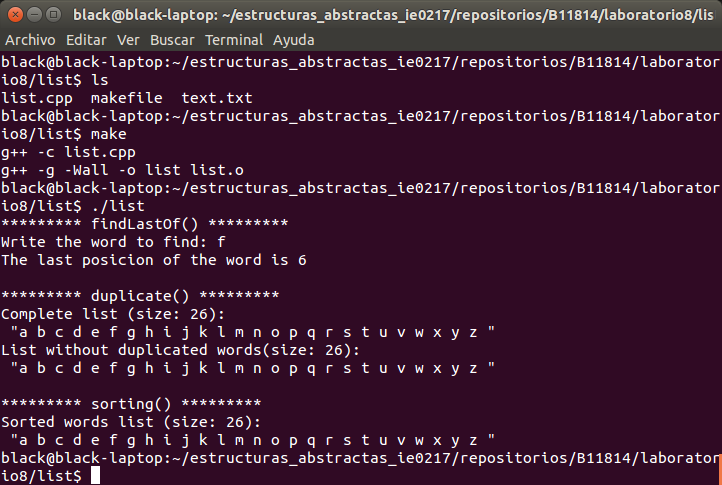
\includegraphics[scale=0.6]{imagenes/list.png}
\label{fig:list}
\end{figure}

\section{Contenedor stack}
En esta parte de laboratorio, se cre\' o una funci\' on llamada \textit{multiBase()}, la cual se encarga simplemente de recibir un numero en base decimal, y pasarlo a otra base especificada por el usuario, entre 2 y 9. Un ejemplo se puede observar en la figura \ref{fig:stack}.
\begin{figure}[hbtp]
\caption{Ejemplo de stack}
\centering
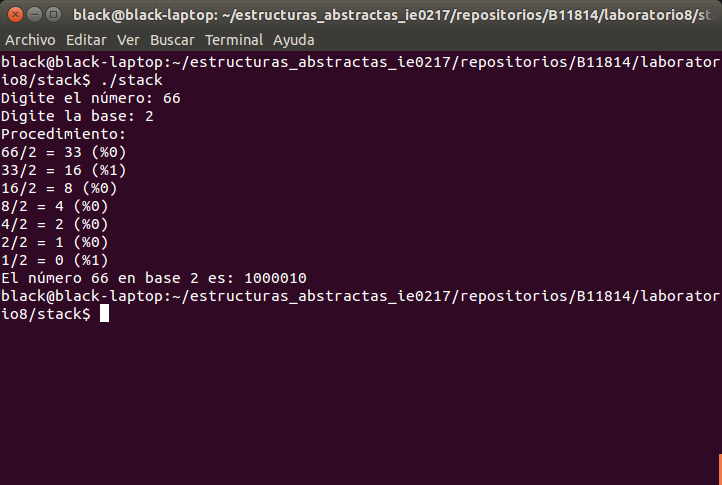
\includegraphics[scale=0.61]{imagenes/stack.png}
\label{fig:stack}
\end{figure}

\section{Contenedor Queue}
Al igual que las anteriores, esta parte se encarga de implementar un algoritmo que utilza \textit{radix sort}, especificamente para ordenar una secuencia de numeros ingresados por el usuario. Un ejemplo se puede observar en la Figura \ref{fig:queue}.

\begin{figure}[hbtp]
\caption{Ejemplo de queue}
\centering
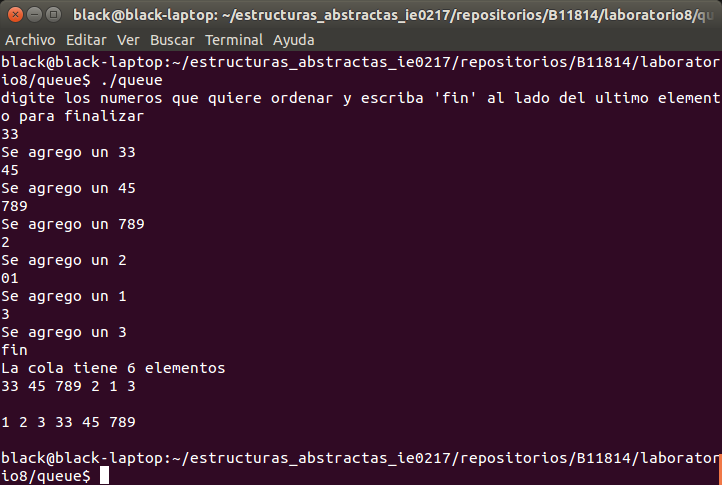
\includegraphics[scale=0.6]{imagenes/queue.png}
\label{fig:queue}
\end{figure}


\section{Contenedor map}
Finalmente, se realiz\' o la implementacion de un contenedor tipo \textit{map}, en cual se encarga de almacenar los n\' umero de carn\' e, nombre del t\' itulo e integrantes de proyecto del curso. 
Uno de los aspectos a destacar es que esta funci\' on o programa tiene que ser capaz de conocer si un carne digitado por el usuario es v\' alido o inv\' alido, y no crashear en el intento.
Por ejemplo, se puede observar la Figura \ref{fig:map}, donde evidentemente se utilzaron numeros de carn\' e ficticios debido al deconocimiento de los mismos.

\begin{figure}[hbtp]
\caption{Uso de map}
\centering
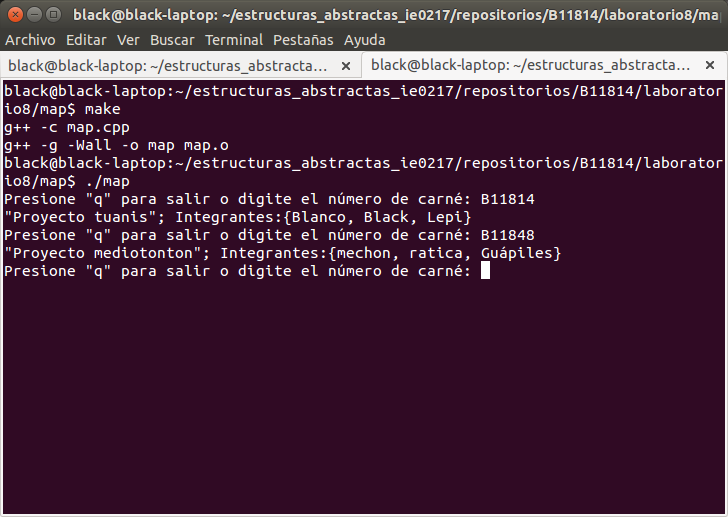
\includegraphics[scale=0.6]{imagenes/map.png}
\label{fig:map}
\end{figure}

\section{Algoritmos}
En C++ los algor\' itmos se refieren a una librer\' ia  que se utiliza para una gran variedad de prop\' ositos, por ejemplo, b\' usquedas, ordenamientoos, cuentas, manipulaci\' on, etc. Siempre se utilzan los \' idices \textit{(first,last)} para definir los rangos. 
En este caso se utiliz\' o el algoritmo \textit{copy}, \textit{sort}, \textit{count}, \textit{accumulate} y \textit{reverse}.

\subsection{Copy}
Copia elementos en el rango definido a otro rango comenzando con d first.

\begin{verbatim}
template<class InputIt, class OutputIt>
OutputIt copy(InputIt first, InputIt last, 
              OutputIt d_first)
{
    while (first != last) {
        *d_first++ = *first++;
    }
    return d_first;
}
\end{verbatim}

\subsection{Sort}
Ordena los elementos en el rango definido en orden ascentente. Si se desea un orden descendente se utilza el par\' ametro \textit{greater}.
Header
\begin{verbatim} 
template< class RandomIt >
void sort( RandomIt first, RandomIt last );
\end{verbatim}
\subsection{Count}
Returna el numero de elementos en el rango definido
\begin{verbatim}
template< class InputIt, class T >

typename iterator_traits<InputIt>::difference_type
    count( InputIt first, InputIt last, const T &value );
    \end{verbatim}
\subsection{Accumulate}
Calcula la suma de valores dados en el rango definido.
\begin{verbatim}
template< class InputIt, class T >
T accumulate( InputIt first, InputIt last, T init );
\end{verbatim}
\subsection{Reverse}
Reordena los elementos del rango definido en orden inverso.
\begin{verbatim}
template< class BidirIt >
void reverse( BidirIt first, BidirIt last );
	
\end{verbatim}

\end{document}
